\chapter{Obtención de la región de interés}
\label{cha:Obtención de la región de interés}

\begin{FraseCelebre}
  \begin{Frase}
    Texto.
  \end{Frase}
  \begin{Fuente}
    Autor texto
  \end{Fuente}
\end{FraseCelebre}

\noindent
La obtención de la posición tridimensional de los objetos del entorno, a partir de unas bounding boxes 2D en una imagen es muy difícil, ya que tiene que ser necesario inferir una tercera dimensión a partir de la dos dimensiones de una imagen. Como se ha visto previamente en la sección \ref{sec:Sistema de proyección de la nube de puntos a la cámara}, donde se presentan las transformaciones necesarias para convertir una escena tridimensional del mundo a una imagen, es posible convertir cualquier punto del entorno en un píxel dentro las imágenes tomadas por la cámara. Estudiando las características de la cámara utilizada para tomar las imágenes, es posible obtener la distancia haciendo el cálculo inverso realizado en la proyección de la nube de puntos del \ac{LiDAR} a la cámara.

Partiendo de las detecciones 2D obtenidas por el modelo YOLOv5m y la distancia a los objetos detectados sobre la imagen, se pretende transformar del sistema de coordenadas pixélicas de la imagen al sistema de coordenadas del mundo según el sistema de coordenadas del \ac{LiDAR}, de esta manera se podría obtener el centro tridimensional de los objetos del entorno que hayan sido detectados y ajustar las \ac{RoI} alrededor de cada objeto para que el proceso de análisis de la nube de puntos sea más sencillo y rápido debido al uso en exclusiva de los puntos que se encuentren sobre los objetos o en una región muy cercana a estos.

La \ac{RoI} que quiere ser definida tiene una forma geométrica de tronco (o frustum) de pirámide de base rectangular, esto es así, ya que si se filtran los puntos del \ac{LiDAR} contenidos dentro de una bounding box 2D de una imagen, se consigue que los puntos del \ac{LiDAR} se encuentren dentro de una pirámide con vértice de la pirámide en la cámara y una altura igual a la distancia máxima de detección del \ac{LiDAR}. Si se consigue obtener la distancia aproximada al objeto a detectar y proyectarla sobre la altura de la pirámide, se puede aplicar un margen de error fijo que sea el mismo obtenido en el modelo de aproximación de la distancia, y con este cortar la pirámide construyendo de esta manera un frustum de la pirámide inicial con los puntos necesarios para el análisis de esa sección de la nube de puntos.

En este capítulo se presentará por tanto el proceso necesario para la transformación de píxeles en las imágenes a puntos tridimensionales en el sistema de coordenadas de la cámara y del \ac{LiDAR}, como los pasos necesarios para la transformación del la nube de puntos a la \ac{RoI} a utilizar definida como los puntos encontrados dentro de un tronce geométrico. Este estudio se puede encontrar en los siguientes archivos: \url{https://github.com/Javier-DlaP/3D-detection-system-lidar-camera/blob/main/Frustum\%20KITTI/Frustum_formulas.ipynb}, \url{https://github.com/Javier-DlaP/3D-detection-system-lidar-camera/blob/main/src/pcl_img_utils.py}.

\section{Proyección de píxeles en la cámara a coordenadas 3D}
\label{sec:Proyección de píxeles en la cámara a coordenadas 3D}

El proceso de transformación de coordenadas pixélicas en una imagen a las coordenadas 3D sobre un sistema de coordenadas diferente, no es algo que se trate de forma normal debido a la necesidad de una tercera dimensión para realizar este proceso, por ello ha sido necesario estudiar en profundidad las transformaciones necesarias para de esta manera hallar las operaciones necesarias para obtener los puntos 3D que se requieren.

Se comienza recordando la fórmula necesaria para la proyección de la nube de puntos a la imagen obtenida, ya que dicha formula es la que se invertirá para obtener los puntos tridimensionales:

\begin{center}
$P = P_2 * R_0\_rect * Tr\_velo\_to\_cam$
\end{center}

Uno de los problemas con los se encuentra, en la necesidad de despejar esta ecuación para las transformaciones de un eje de coordenadas a otro, pero mientras que la matriz $R_0\_rect$ es una matriz cuadrada, las matrices $P2$ y $Tr\_velo\_to\_cam$ con matrices no cuadradas, por lo que la inversión de ambas matrices no puede ser perfecta. Debido a esto se han analizado las funciones de ofrecidas por la librería de NumPy de Python, para ver la precisión en la inversión de las matrices además de para comprender de que manera se obtienen las inversiones más precisas, si realizándolas por separado o de forma conjunta.

\begin{center}
$
P * (inv(P_2 * R_0\_rect * Tr\_velo\_to\_cam)) =
\begin{bmatrix}
1.00000e^{+00} & 1.25767e^{-16} & 1.13686e^{-13} \\
1.04083e^{-16} & 1.00000e^{+00} & -1.42108e^{-13} \\
7.52165e^{-19} & -6.06475e^{-19} & 1.00000e^{+00} \\
\end{bmatrix}
$
\end{center}

\begin{center}
$
P * (inv(Tr\_velo\_to\_cam) * inv(R_0\_rect) * inv(P_2)) =
\begin{bmatrix}
1.00000e^{+00} & -3.64291e^{-17} & 1.13686e^{-13} \\
-6.93889e^{-17} & 1.00000e^{+00} & -8.88178e^{-14} \\
-3.38813e^{-21} & 8.90893e^{-19} & 1.00000e^{+00} \\
\end{bmatrix}
$
\end{center}

Como se observa en las en las matrices anteriores, ambas son muy similares a la matriz identidad con un error máximo de $10^{-13}$, lo cual es un error despreciable, por lo que ambas formas de invertir las matrices son igual de válidas.

Observando las matrices que componen el proceso de proyección de la nube de puntos a la cámara, se encuentra que es en el paso del sistema de coordenadas de la cámara a las coordenadas pixélicas de la imagen. En la siguiente fórmula se puede ver como únicamente resolviendo el problema que supone el desconocimiento de $w$, se podría multiplicar por las matrices inversas de $P_2$, $R_0\_rect$ y $Tr\_velo\_to\_cam$ y obtener directamente las coordenadas tridimensionales en el sistema de coordenadas del \ac{LiDAR}.

\begin{center}
$
\begin{bmatrix}
w * x_{1i}\\w * y_{1i}\\w
\end{bmatrix}
= T_{v2c}^{-1} * R_0^{-1} * P_2^{-1}*
\begin{bmatrix}
x_{1l}\\y_{1l}\\z_{1l}\\1
\end{bmatrix}
$
\end{center}

El paso del sistema de coordenadas del \ac{LiDAR} al sistema de la cámara rectificada es tan simple como multiplicar por las matrices $R_0\_rect$ y $Tr\_velo\_to\_cam$, por ello es muy importante obtener un valor de $w$ muy preciso y así poder pasar directamente, con multiplicaciones de matrices que ya se tienen, de un sistema de coordenadas a otro sin ningún problema.

La obtención de la variable $w$ es muy importante, ya que junto con las coordenadas pixélicas ($x_{1i}$, $y_{1i}$), componen la matriz de entrada que permite transformar de vuelta un píxel a su posición en el mundo original. Observando esto se comprende que dicha variable $w$ tiene una relación directa con la distancia a la que se quiere proyectar dicho píxel, para ello se define el sistema cuatro ecuaciones que relacionan todas las incógnitas y que permite la obtención de la variable $w$.

\begin{center}
$PRT = P_2 * R_0\_rect * Tr\_velo\_to\_cam$
\end{center}

\begin{center}
$w * x_{1i} = PRT_{0,0} * x_{1l} + PRT_{0,1} * y_{1l} + PRT_{0,2} * z_{1l} + PRT_{0,3}$\\
$w * y_{1i} = PRT_{1,0} * x_{1l} + PRT_{1,1} * y_{1l} + PRT_{1,2} * z_{1l} + PRT_{1,3}$\\
$w * z_{1i} = PRT_{2,0} * x_{1l} + PRT_{2,1} * y_{1l} + PRT_{2,2} * z_{1l} + PRT_{2,3}$\\
$d = \sqrt{x_{1l}^2 + y_{1l}^2 + z_{1l}^2}$
\end{center}

Este sistema de cuatro ecuaciones con cuatro incógnitas se basa en el desconocimiento de la variable $w$ además de las coordenadas tridimensionales de los puntos que se quieren obtener ($x_{1l}$, $y_{1l}$, $z_{1l}$), la aplicación de la multiplicación de matrices y la aplicación la formula de la distancia entre dos puntos tridimensionales. De esta manera resolviendo este sistema de coordenadas se puede obtener el valor de $w$ o directamente tratar con los puntos 3D en el sistema de coordenadas del \ac{LiDAR}.

Para solucionar este sistema de ecuaciones se ha calculando la matriz $PRT$ y se ha tratado de resolver el sistema de forma tradicional, pero al ser un sistema de ecuaciones tan complejo y debido a la fórmula de la distancia con la raíz cuadrada y las potencias, ha sido muy difícil de completar, además de que más tarde se ha observado de que en ciertas escenas del dataset, las cámaras y su posición son modificadas, por lo que tampoco se podría utilizar. Debido a ello se ha terminado utilizando la librería SciPy para resolver en tiempo real el sistema de ecuaciones, lo cual añadirá tiempo al sistema de detección 3D completo, pero por ahora se ha terminado utilizando, ya que la función de resolución del sistema de ecuaciones logra como como mucho un error $10^{-12}$ lo cual es despreciable.

\section{Obtención del tronco geométrico}
\label{sec:Obtención del tronco geométrico}

Tras la obtención de la proyección de los píxeles sobre el sistema de coordenadas del \ac{LiDAR} como puntos tridimensionales, se trata de obtener la \ac{RoI} con los puntos más cercanos al objeto que se quiere detectar, para ello se va a realizar un proceso en el que la nube de puntos: se filtrará según las bounding boxes obtenidas, se rotará la nube de puntos para que el objeto se encuentre sobre el eje Y, se trasladará al origen de coordenadas para el procesamiento por parte del modelo neuronal de la misma región del espacio y por último se filtrará según el error del modelo de aproximación de la distancia.

Siendo este un proceso poco claro si se realiza de forma explicativa únicamente, se han elegido dos casos sencillos en los que únicamente se trata con un objeto como ocurre en las situaciones de la Figura \ref{fig:Nubes de puntos de KITTI con su ground-truth.}, de esta manera se puede observar en múltiples casos, todo el procesamiento que se realiza sobre todos los objetos que son detectados sobre la cámara.

\begin{figure}[H]
	\begin{minipage}{0.495\textwidth}
		\centering
		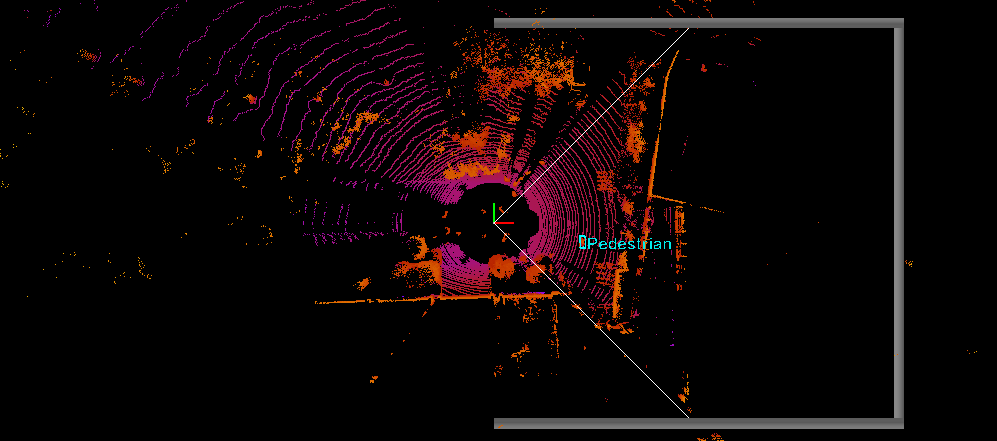
\includegraphics[width=1\linewidth]{Book/figures/7_roi/kitti_pcl_0.png}
	\end{minipage}\hfill
	\begin{minipage}{0.495\textwidth}
		\centering
		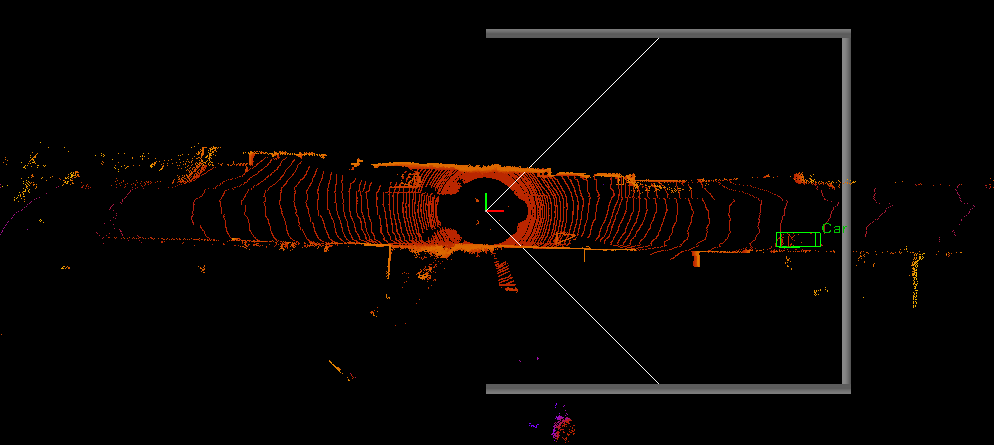
\includegraphics[width=1\linewidth]{Book/figures/7_roi/kitti_pcl_2.png}
	\end{minipage}
	\caption{Nubes de puntos de KITTI con su ground-truth.}
	\label{fig:Nubes de puntos de KITTI con su ground-truth.}
\end{figure}

El primero de los pasos a realizar es el filtrado de la nube de puntos, de forma que por cada objeto del entorno se utilizan únicamente los puntos del \ac{LiDAR} que se encuentran dentro de las bounding boxes 2D correspondientes a la salida del modelo YOLOv5m. Para ello se comenzó probando con la creación de una pirámide tridimensional mediante la proyección en forma de arista (por lo que no hace falta la distancia) de cada uno de los vértices de los que se compone cada detección 2D, y tras esto se analizaba los puntos que se encontraban dentro de dicha pirámide de base rectangular. El problema con este método, es el tiempo que tarda en ejecutarse teniendo en cuenta que se tiene que aplicar por cada objeto detectado, por ello, se ha definido otro método para la obtención de las nubes de puntos filtradas.

En el método utilizado, se obtienen los puntos pertenecientes a las bounding boxes a partir del uso de múltiples máscaras, las cuales son calculadas mediante la nube de puntos proyectada en la imagen (previamente calculada) y las detecciones 2D, a partir de estas máscaras se consigue obtener directamente las diferentes nubes de puntos mediante la aplicación de las máscaras sobre la nube de puntos original. Además, en dicho filtrado se tiene en cuenta la distancia a los objetos, ya que gracias a dichas distancias, se puede eliminar las regiones de la nube de puntos de un objeto que se encuentre detrás de otro, para que de esta manera el objeto que este más alejado sea detectado y no haya confusión con los puntos del objeto más próximo. Con este método se consigue obtener las nubes de puntos filtradas en las que se encuentran únicamente los objetos a detectar posteriormente de forma tridimensional como se ve en la Figura \ref{fig:Nubes de puntos de KITTI filtradas por las detecciones 2D.}.

\begin{figure}[H]
	\begin{minipage}{0.495\textwidth}
		\centering
		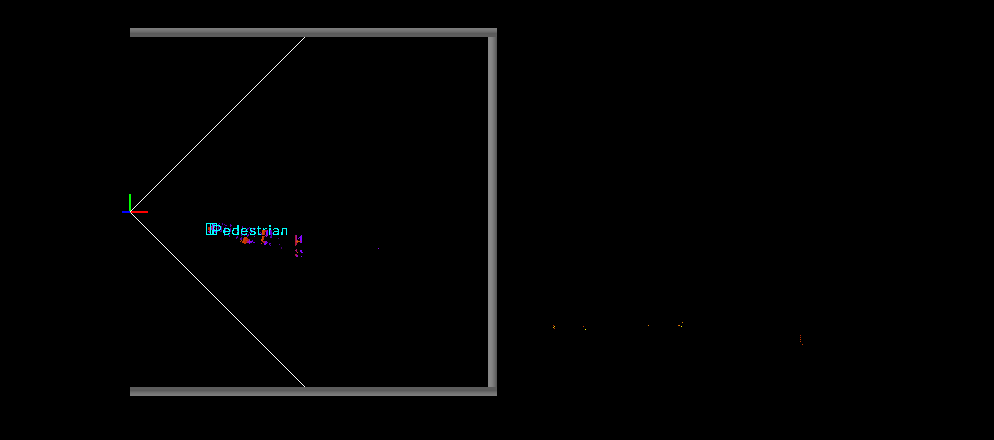
\includegraphics[width=1\linewidth]{Book/figures/7_roi/kitti_pcl_filt_0.png}
	\end{minipage}\hfill
	\begin{minipage}{0.495\textwidth}
		\centering
		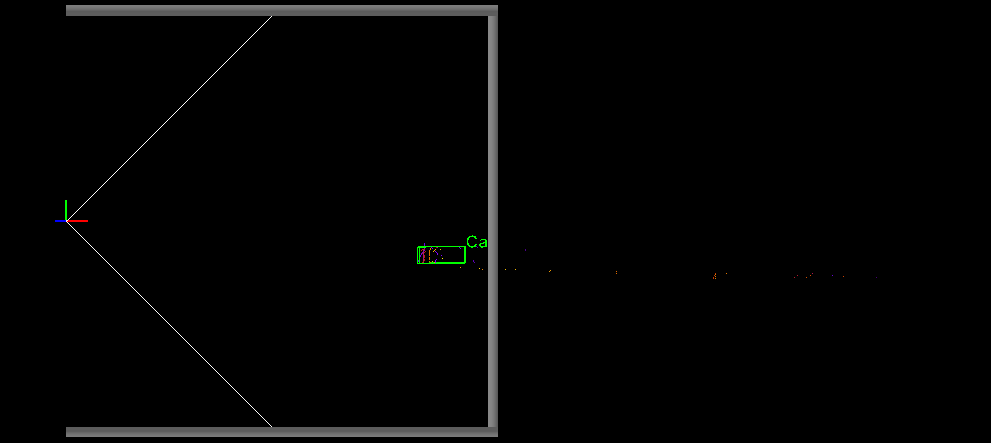
\includegraphics[width=1\linewidth]{Book/figures/7_roi/kitti_pcl_filt_2.png}
	\end{minipage}
	\caption{Nubes de puntos de KITTI filtradas por las detecciones 2D.}
	\label{fig:Nubes de puntos de KITTI filtradas por las detecciones 2D.}
\end{figure}

De forma similar a como se realiza en el modelo Frustum PointNets visto en la Sección \ref{sec:Frustum PointNets}, los objetos detectados se rotan a la parte frontal del vehículo, lo que es el eje Y en el sistema de coordenadas del \ac{LiDAR}, para de esta manera reducir la región de análisis por un modelo de detección 3D, ya que suelen usar un volumen situado una posición concreta como la región de ejecución del algoritmo.

\begin{center}
$\alpha = - \arctan(x_{1l}, z_{1l})$
\end{center}
\begin{center}
$
\begin{bmatrix}
x_{1lr}\\y_{1lr}\\z_{1lr}\\1
\end{bmatrix}
=
\begin{bmatrix}
\cos{\alpha}&0&\sin{\alpha}&0\\
0&1&0&0\\
-\sin{\alpha}&0&\cos{\alpha}&0\\
0&0&0&1\\
\end{bmatrix}
\begin{bmatrix}
x_{1l}\\y_{1l}\\z_{1l}\\1
\end{bmatrix}
$
\end{center}

La ejecución de este algoritmo se basa en la posición 3D del objeto que ha sido obtenido previamente, pero que no se ve afectado por un fallo en la distancia aproximada, ya que cualquier distaría sería suficiente para obtener el ángulo de rotación y aplicar la matriz de rotación sobre el eje Y del centro aproximado del objeto a detectar junto con la nube de puntos con la que se trabaja. Es necesario tener en cuenta que mediante la rotación de la nube de puntos, se ha rotado también la dirección del vehículo en la misma proporción, ya que más adelante será necesario revertir este giro para obtener la posición 3D original del objeto. Los resultados de esta transformación se observan en la Figura \ref{fig:Nubes de puntos de KITTI rotadas al eje Y.}.

\begin{figure}[H]
	\begin{minipage}{0.495\textwidth}
		\centering
		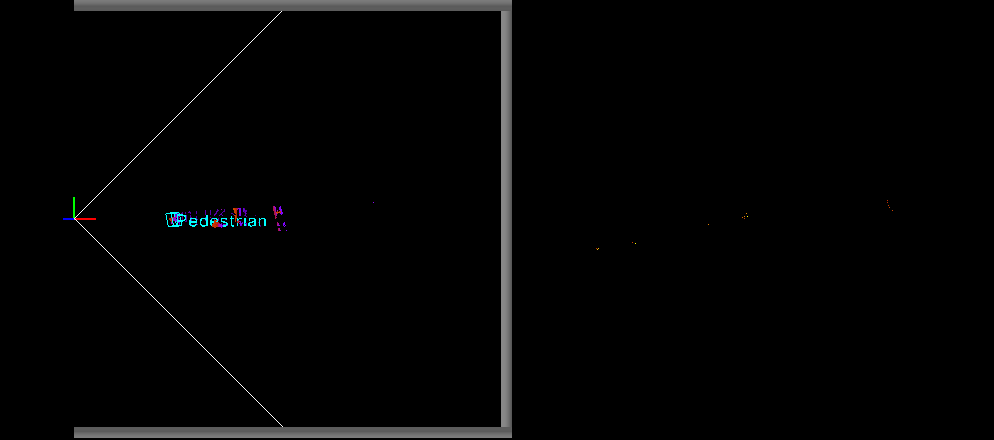
\includegraphics[width=1\linewidth]{Book/figures/7_roi/kitti_pcl_rot_0.png}
	\end{minipage}\hfill
	\begin{minipage}{0.495\textwidth}
		\centering
		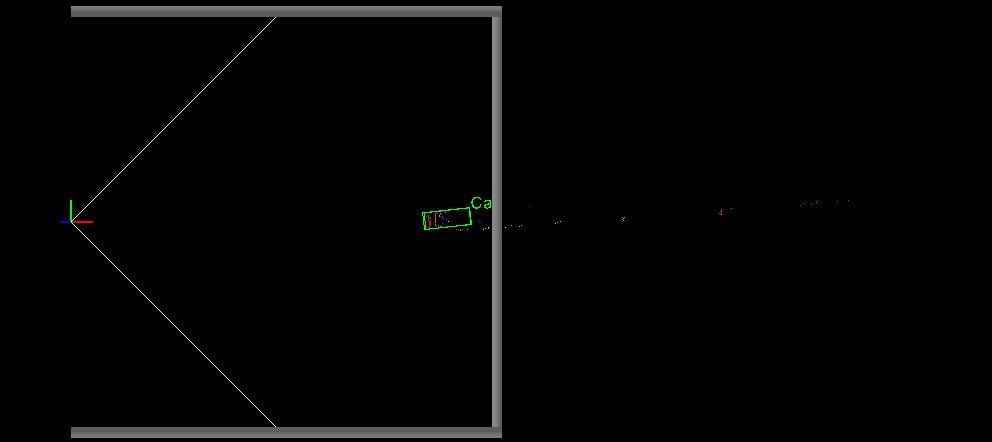
\includegraphics[width=1\linewidth]{Book/figures/7_roi/kitti_pcl_rot_2.png}
	\end{minipage}
	\caption{Nubes de puntos de KITTI rotadas sobre el eje Y.}
	\label{fig:Nubes de puntos de KITTI rotadas al eje Y.}
\end{figure}

El siguiente paso, es la traslación del objeto de interés y de la nube de puntos al origen de coordenadas, de esta manera se podrá analizar la nube de puntos exclusivamente en el origen de coordenadas y no será necesario estudiar el resto del entorno como ocurría hasta ahora. Esta traslación se realiza sobre el eje X, de manera que error en la altura del objeto no se ve afecta por esta traslación, ya que la mayoría de escenarios son en superficies planas (todas en este dataset), y se ve bastante afectado un fallo en el calculo de la distancia al obtener el centro tridimensional del objeto, ya que puede aparecer dicho objeto por encima del resto de objetos o por debajo del suelo, debido a esto solo se traslada en el eje X. La nube de puntos trasladada obtiene resultados como los de la Figura \ref{fig:Nubes de puntos de KITTI movidas al origen de coordenadas.}.

\begin{figure}[H]
	\begin{minipage}{0.495\textwidth}
		\centering
		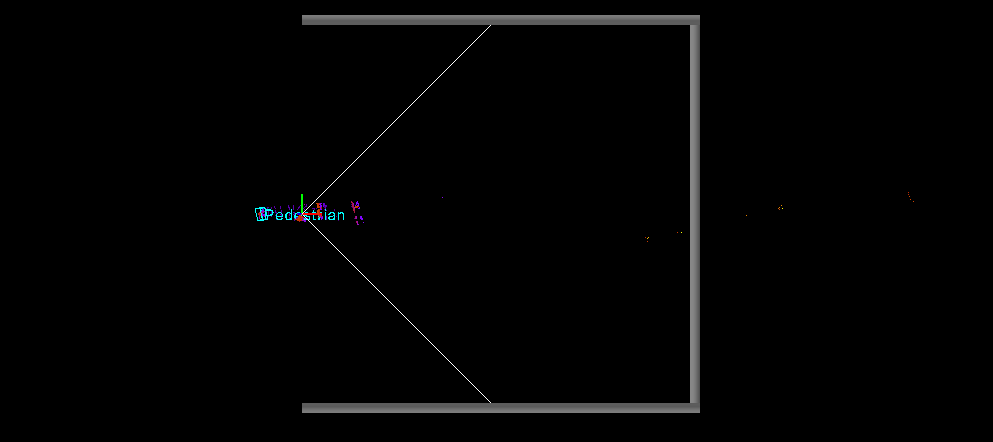
\includegraphics[width=1\linewidth]{Book/figures/7_roi/kitti_pcl_mov_0.png}
	\end{minipage}\hfill
	\begin{minipage}{0.495\textwidth}
		\centering
		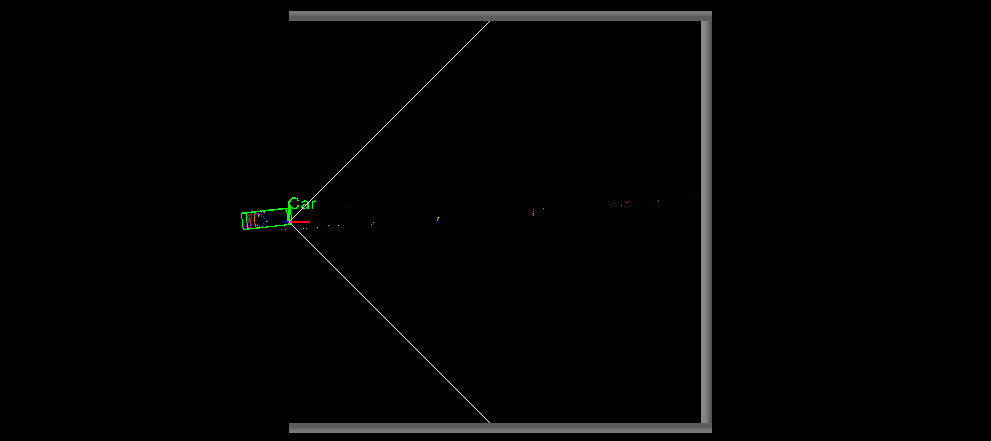
\includegraphics[width=1\linewidth]{Book/figures/7_roi/kitti_pcl_mov_2.png}
	\end{minipage}
	\caption{Nubes de puntos de KITTI movidas al origen de coordenadas.}
	\label{fig:Nubes de puntos de KITTI movidas al origen de coordenadas.}
\end{figure}

Como última fase del proceso de creación del frustum, se elimina el resto de puntos que no se encuentran cerca al objeto de interés, por lo que los dos planos que se crean para cortar la pirámide en la que se encuentran los puntos del \ac{LiDAR} son perpendiculares al eje X. La distancia a la que se crean dichos planos es igual al rango de confianza que se ha definido para el modelo de error de la distancia, por lo que gracias a este filtrado se eliminan lo puntos que se observaban de forma lejana al objeto de interés en la figura anterior. Como se ve en la Figura \ref{fig:Frustums obtenidos a partir de las nubes de puntos de KITTI.}, este filtrado final de los puntos más alejados deja únicamente a los puntos que se encuentran más cerca del objeto, por lo que es más sencilla su detección a posteriori.

\begin{figure}[H]
	\begin{minipage}{0.495\textwidth}
		\centering
		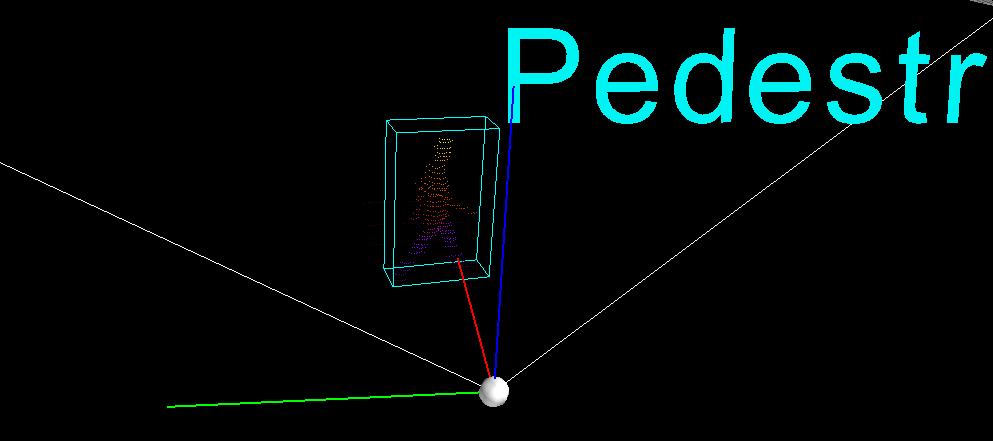
\includegraphics[width=1\linewidth]{Book/figures/7_roi/kitti_pcl_frustum_0.png}
	\end{minipage}\hfill
	\begin{minipage}{0.495\textwidth}
		\centering
		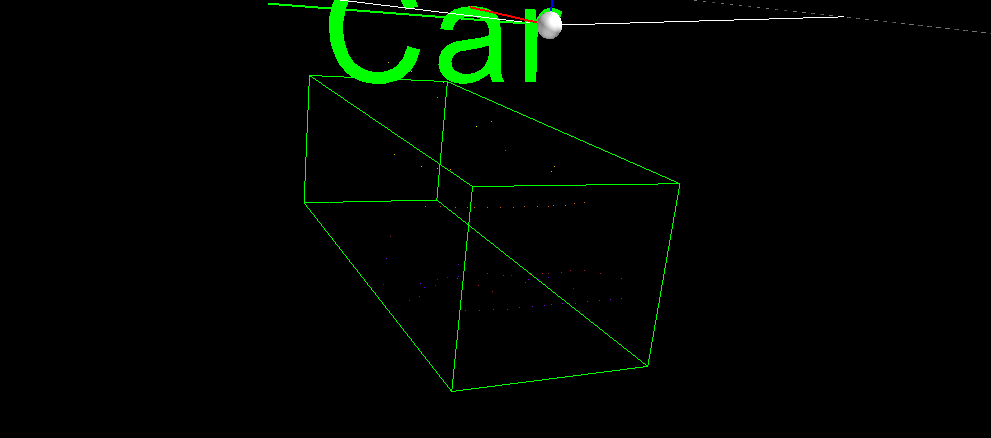
\includegraphics[width=1\linewidth]{Book/figures/7_roi/kitti_pcl_frustum_2.png}
	\end{minipage}
	\caption{Frustums obtenidos a partir de las nubes de puntos de KITTI.}
	\label{fig:Frustums obtenidos a partir de las nubes de puntos de KITTI.}
\end{figure}

Dentro de las figuras mostradas se puede observar como los objetos no han terminado en el centro del sistema de coordenadas, esto no es debido a un error en la programación de las transformaciones geométricas, sino que para simular el error del sistema completo, se ha añadido un error a los bordes de las cajas 2D y a la distancia de forma similar. Este proceso de simulación del error del sistema completo se explicará en la Sección \ref{sec:Entrenamiento y evaluación de Frustum PointPillars}, ya que tiene gran importancia en la creación del modelo de detección 3D basado en \ac{LiDAR}.